\documentclass{article}
\usepackage{graphicx}

\begin{document}
\title{Comparison of Epitopes and paratopes}

\author{Miruna Serian}
\date{2019}
\maketitle
\newpage 

\section*{Abstract}
\markright{}
This is the abstract
\section{Introduction}
\markright{}
\newpage 
\section{Methods}
\subsection{Identifying Ig/Ag complexes}
 72 Ig/Ag complexes associated with lysozyme where identified using IMGT's database. The antigens from the obtained complexes come from different species: Camelus dromedarius(14 complexes), shark - Ginglymostoma cirratum(4 complexes), mouse - Mus musculus (53 complexes). Three out of the complexes contain humanized antibodies.
 
\subsection{Retrieving contacts}
Annotation for the antibody and lysozyme chains for each pdb entry was obtained from the IMGT and was further used to collect information about the interactions between the antigen chain and both heavy and light chains from the antibody. The interacting residues' positions and their names were fetched from PDBSum and stored locally.

\subsection{CDR extraction and filtering}

A Multiple Sequence Alignment of the antibody structures present in the Ab-Ag complexes revealed that many of these complexes were redundant in the sense that they included numerous representatives of the same protein, for example as site-specific mutants.  For the purpose od this Ab/Ag interaction comparison, all but one Ag–Ab complex representative of a unique CDR were deleted from the data set.
 \\
The CDR sequences for both heavy and light chains for each antibody in the Ag/Ig complexes were extracted from PyIgClassify: a database of antibody CDR structural classifications using a script wrote in python. The overall similarity of the CRDs as well as for each type of CDR between the Abs was compared using similarity scores. The algorithm for generating the similarity scores uses an averaged string matching score computed for each pair of CDRs from two different Abs pair in the dataset. 
For the purpose of this paratope-epitope comparison, the complexes containing antibodies with identical overall CDRs were filtered out for further analyses.

\subsection{Epitope identification}
For the lysozyme chain in each complex, the amino acid sequences were downloaded using pdb-tools[] and were further aligned using EBI' Clustal Omega MSA tool. The generated alignment was downloaded and a script was used to obtain the equivalent contact positions for every sequence which takes into account the insertions and gaps. For each of the complexes with unique CDR antibodies, the equivalent contact residues on each Ag chain and their frequency were then plotted onto a heatmap for first observations of the epitope. 


For an initial ovrepresentation of the epitopes in the data, a heatmap was used to plot the Ag residues that interact with Abs through both hydrogen bonds and non hydrogen bonds and their respective number of contacts.
\begin{figure}[h]
	\centering
	\includegraphics[width=0.7\linewidth]{plots_new_gr/epitope_no_contacts_unique_all_pdbs_all_all}
	\caption{}
	\label{fig:epitopenocontactsuniqueallpdbsallall}
\end{figure}


To analyse the similarity between the lysozyme epitope in each of the complexes with unique Ab CDRs, the Jaccard index was computed for each pair of epitopes(antigen contact residues positions represented as numbers) and the average for each complex was plotted(Fig.1 ). The Jaccard similarity coefficient is defined as the size of the intersection divided by the size of the union of two sets and can serve as an useful measure of similarity for  two sets of data, with a range from 0 to 100. 
\begin{figure}[h]
	\centering
	\includegraphics[width=0.5\linewidth]{unique_cdr_barplot_jaccard}
	\caption[Jaccrad index]{}
	\label{fig:uniquecdrbarplotjaccard}
\end{figure}


Based on the distribution of the Jaccard scores as well as an overall comparison of epitope contacts across all complexes, 3 groups of similar epitopes were defined with different species composition.
\begin{figure}[h]
	\centering
	\includegraphics[width=0.95\linewidth]{plots_new_gr/group_composition}
	\caption{}
	\label{fig:groupcomposition}
\end{figure}

\\
\begin{tabular}{llll}{}
	\toprule
	{} &     I &    II &   III \\
	\hline
	\midrule
	0  &  2dqd &  1ri8 &  1jto \\
	1  &  1xgr &  1bql &  1jtp \\
	2  &  1xgt &  2iff &  1jtt \\
	3  &  1xgq &  1mlc &  1rjc \\
	4  &  1dqj &  1zv5 &  1xfp \\
	5  &  2dqc &   &  1zmy \\
	6  &  1c08 &   &  1t6v \\
	7  &  1xgu &   &  1sq2 \\
	8  &  1ic5 &   &  2i25 \\
	9  &  1ic4 &   &  2i26 \\
	10 &  1ic7 &   &   \\
	11 &  2dqh &   &   \\
	12 &  1ua6 &   &   \\
	13 &  1xgp &   &   \\
	14 &  2dqe &   &   \\
	15 &  2dqg &   &   \\
	\bottomrule
\end{tabular}

\\

\section{Results}
\subsection{Epitope binding}

For each of the 3 groups the number of contacts(hydrogen bonds and non hydrogen bonds) was plotted. An overall epitope overlap is observed within all groups, with Group 1 having the most similar epitopes. While Group 2 and 3 contain complexes for which the distribution of the contacts have a different pattern, there are some key interacting epitope residues which seem to be conserved within groups.
\begin{figure}[h]
	\centering
	\includegraphics[width=0.7\linewidth]{plots_new_gr/epitope_no_contacts_unique_all_pdbs_all_non_h_bonded}
	\caption{}
	\label{fig:epitopenocontactsuniqueallpdbsallnonhbonded}
\end{figure}
\\


Some of the residues in the epitope were observed to bind more than one position in the antibody. To analyse the pattern of binding, a consensus residue was determined for each position based on the occurrence of residues. Further, for each contacting residue was then assigned a score  of  -1, 0, 1 according to the following criteria:
\begin{itemize}
 \item -1 if the antigen residue is different to consensus 
\item  0 if the epitope residue is binding to multiple residues on the antigen, including the consensus
\item 1 if the epitope residue only binds the consensus

\end{itemize}

\\
Further on, the change in paratope residue preference was compared with the epitope-CDR binding pattern. Across each group, both the paratope residue preference and the CDR binding preference are greatly more varied in the heavy chain, whith the light chain showing conservation.

\begin{figure}[hH]
	\centering
	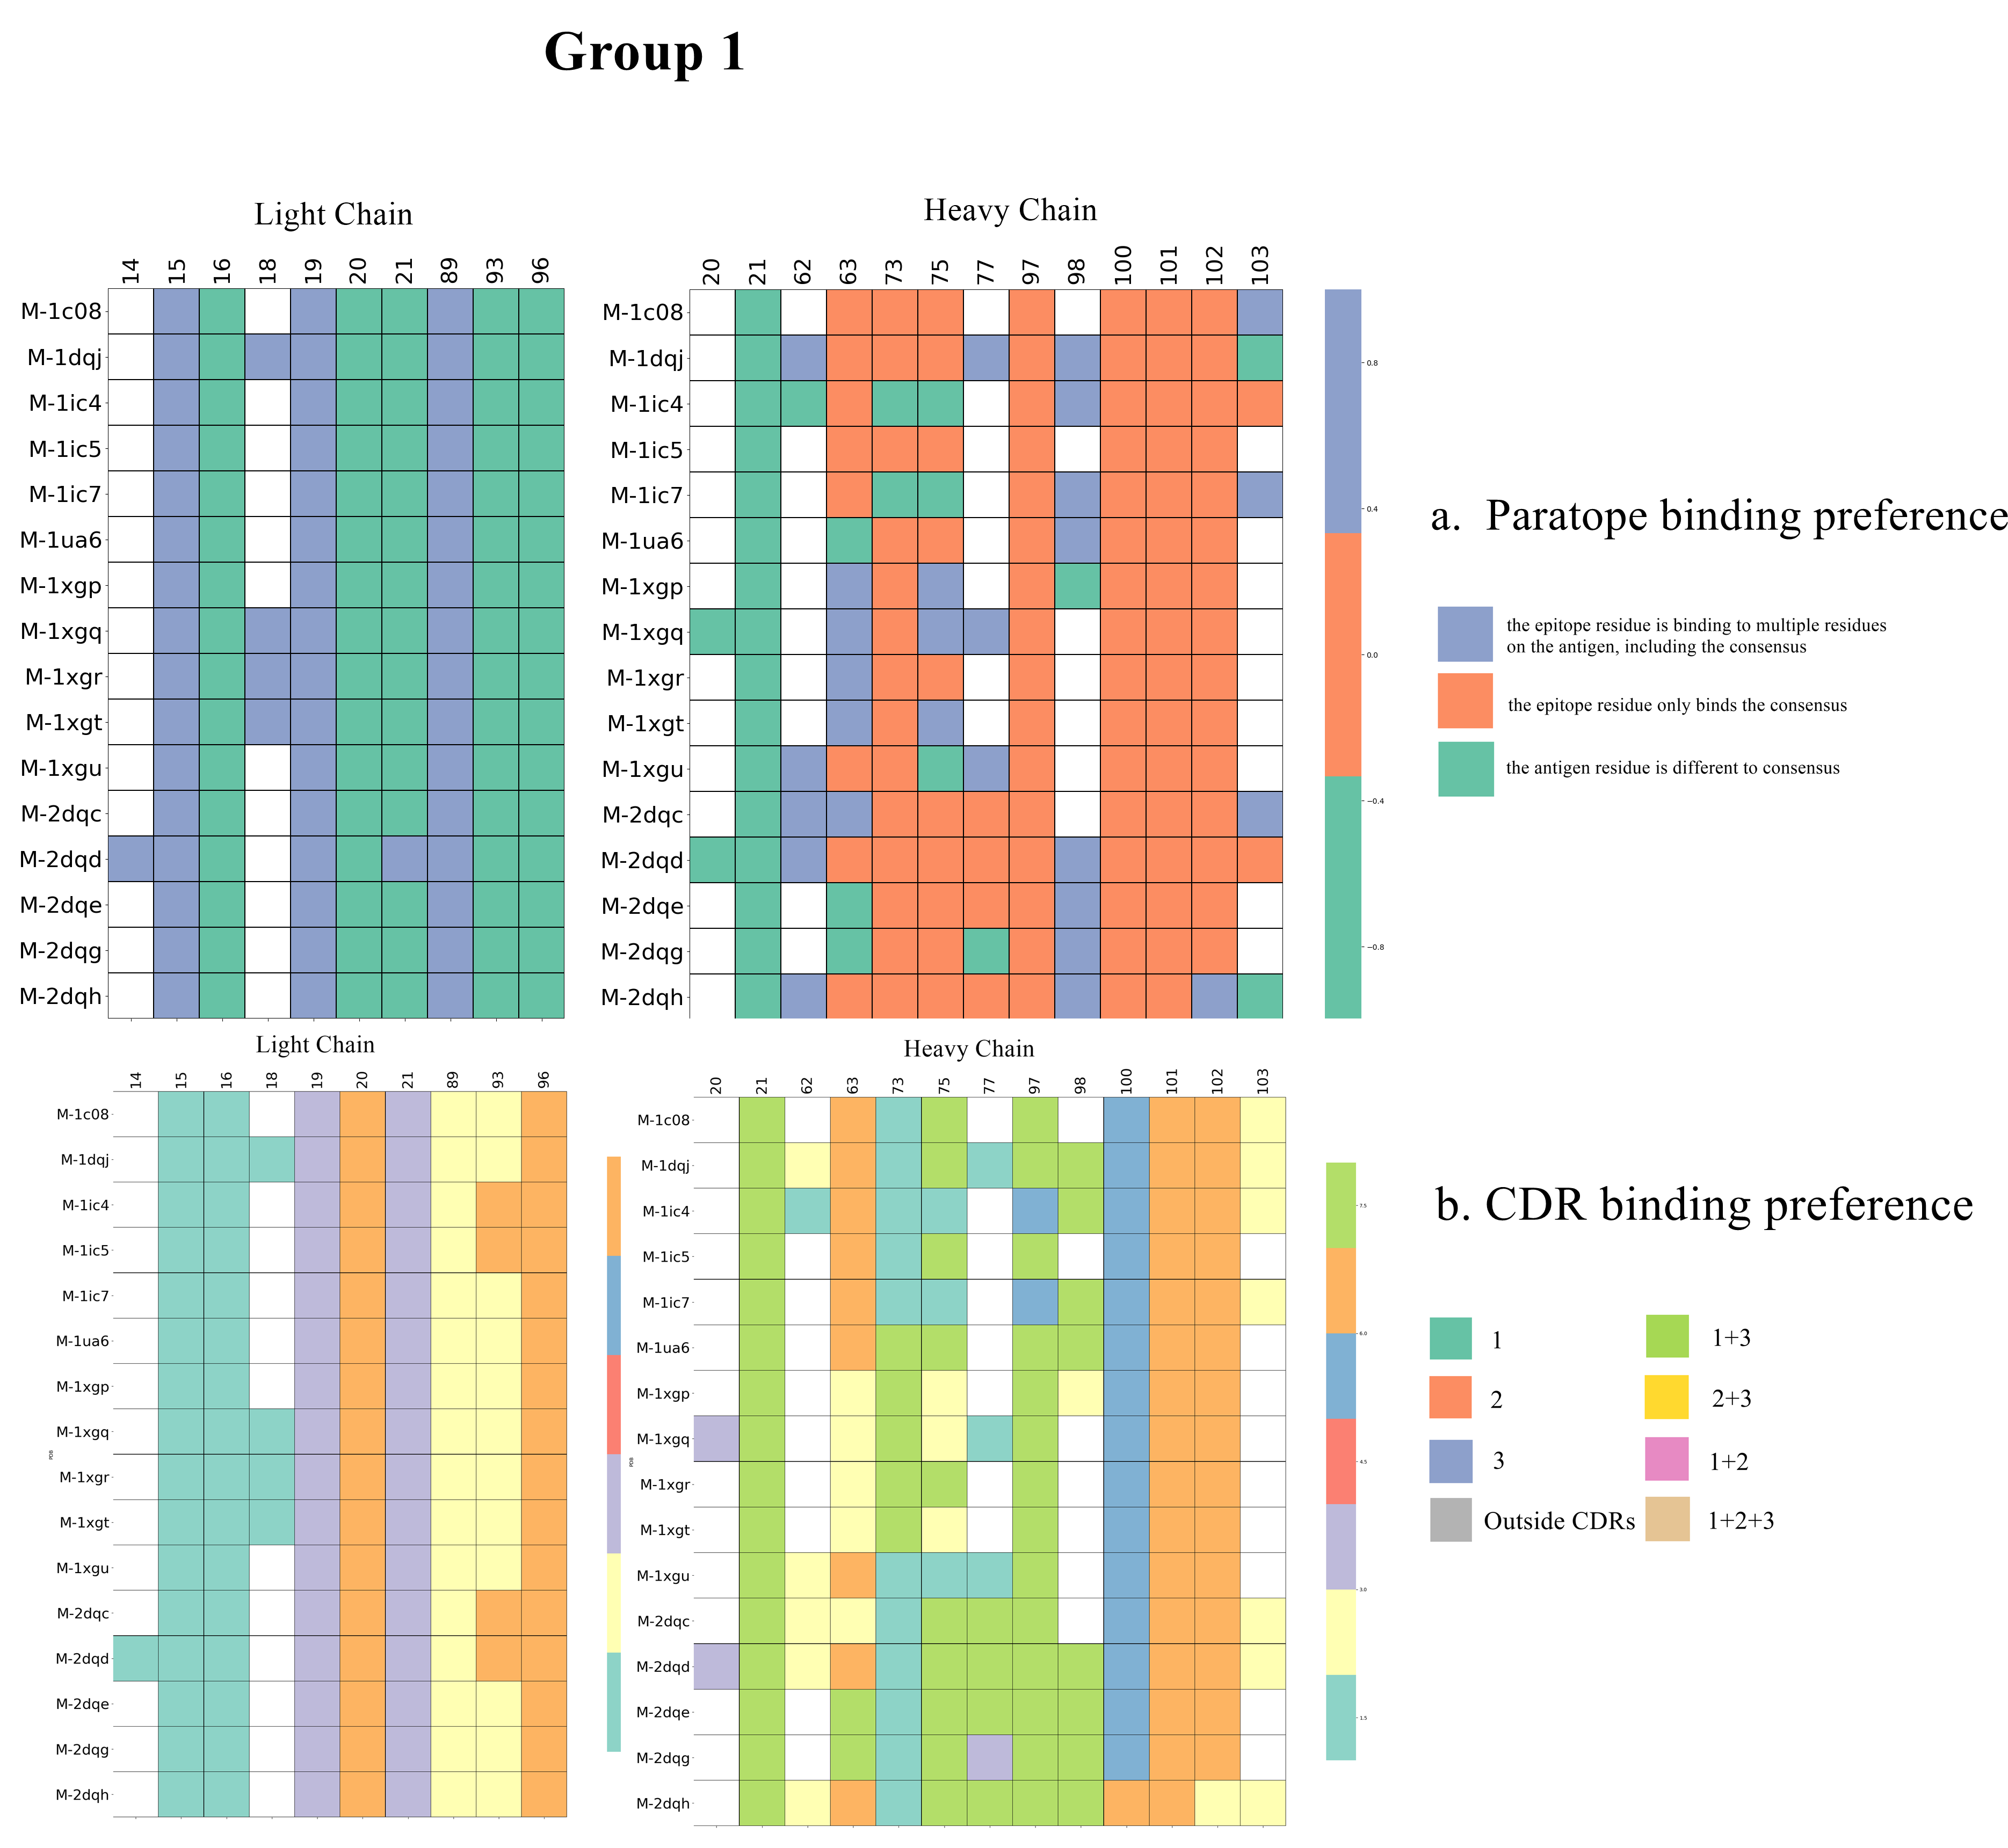
\includegraphics[width=0.7\linewidth]{plots_new_gr/g1_light_vs_heavy_101_vs_cdr}
	\caption{}
	\label{fig:g1lightvsheavy101vscdr}
\end{figure}

\begin{figure}
	\centering
	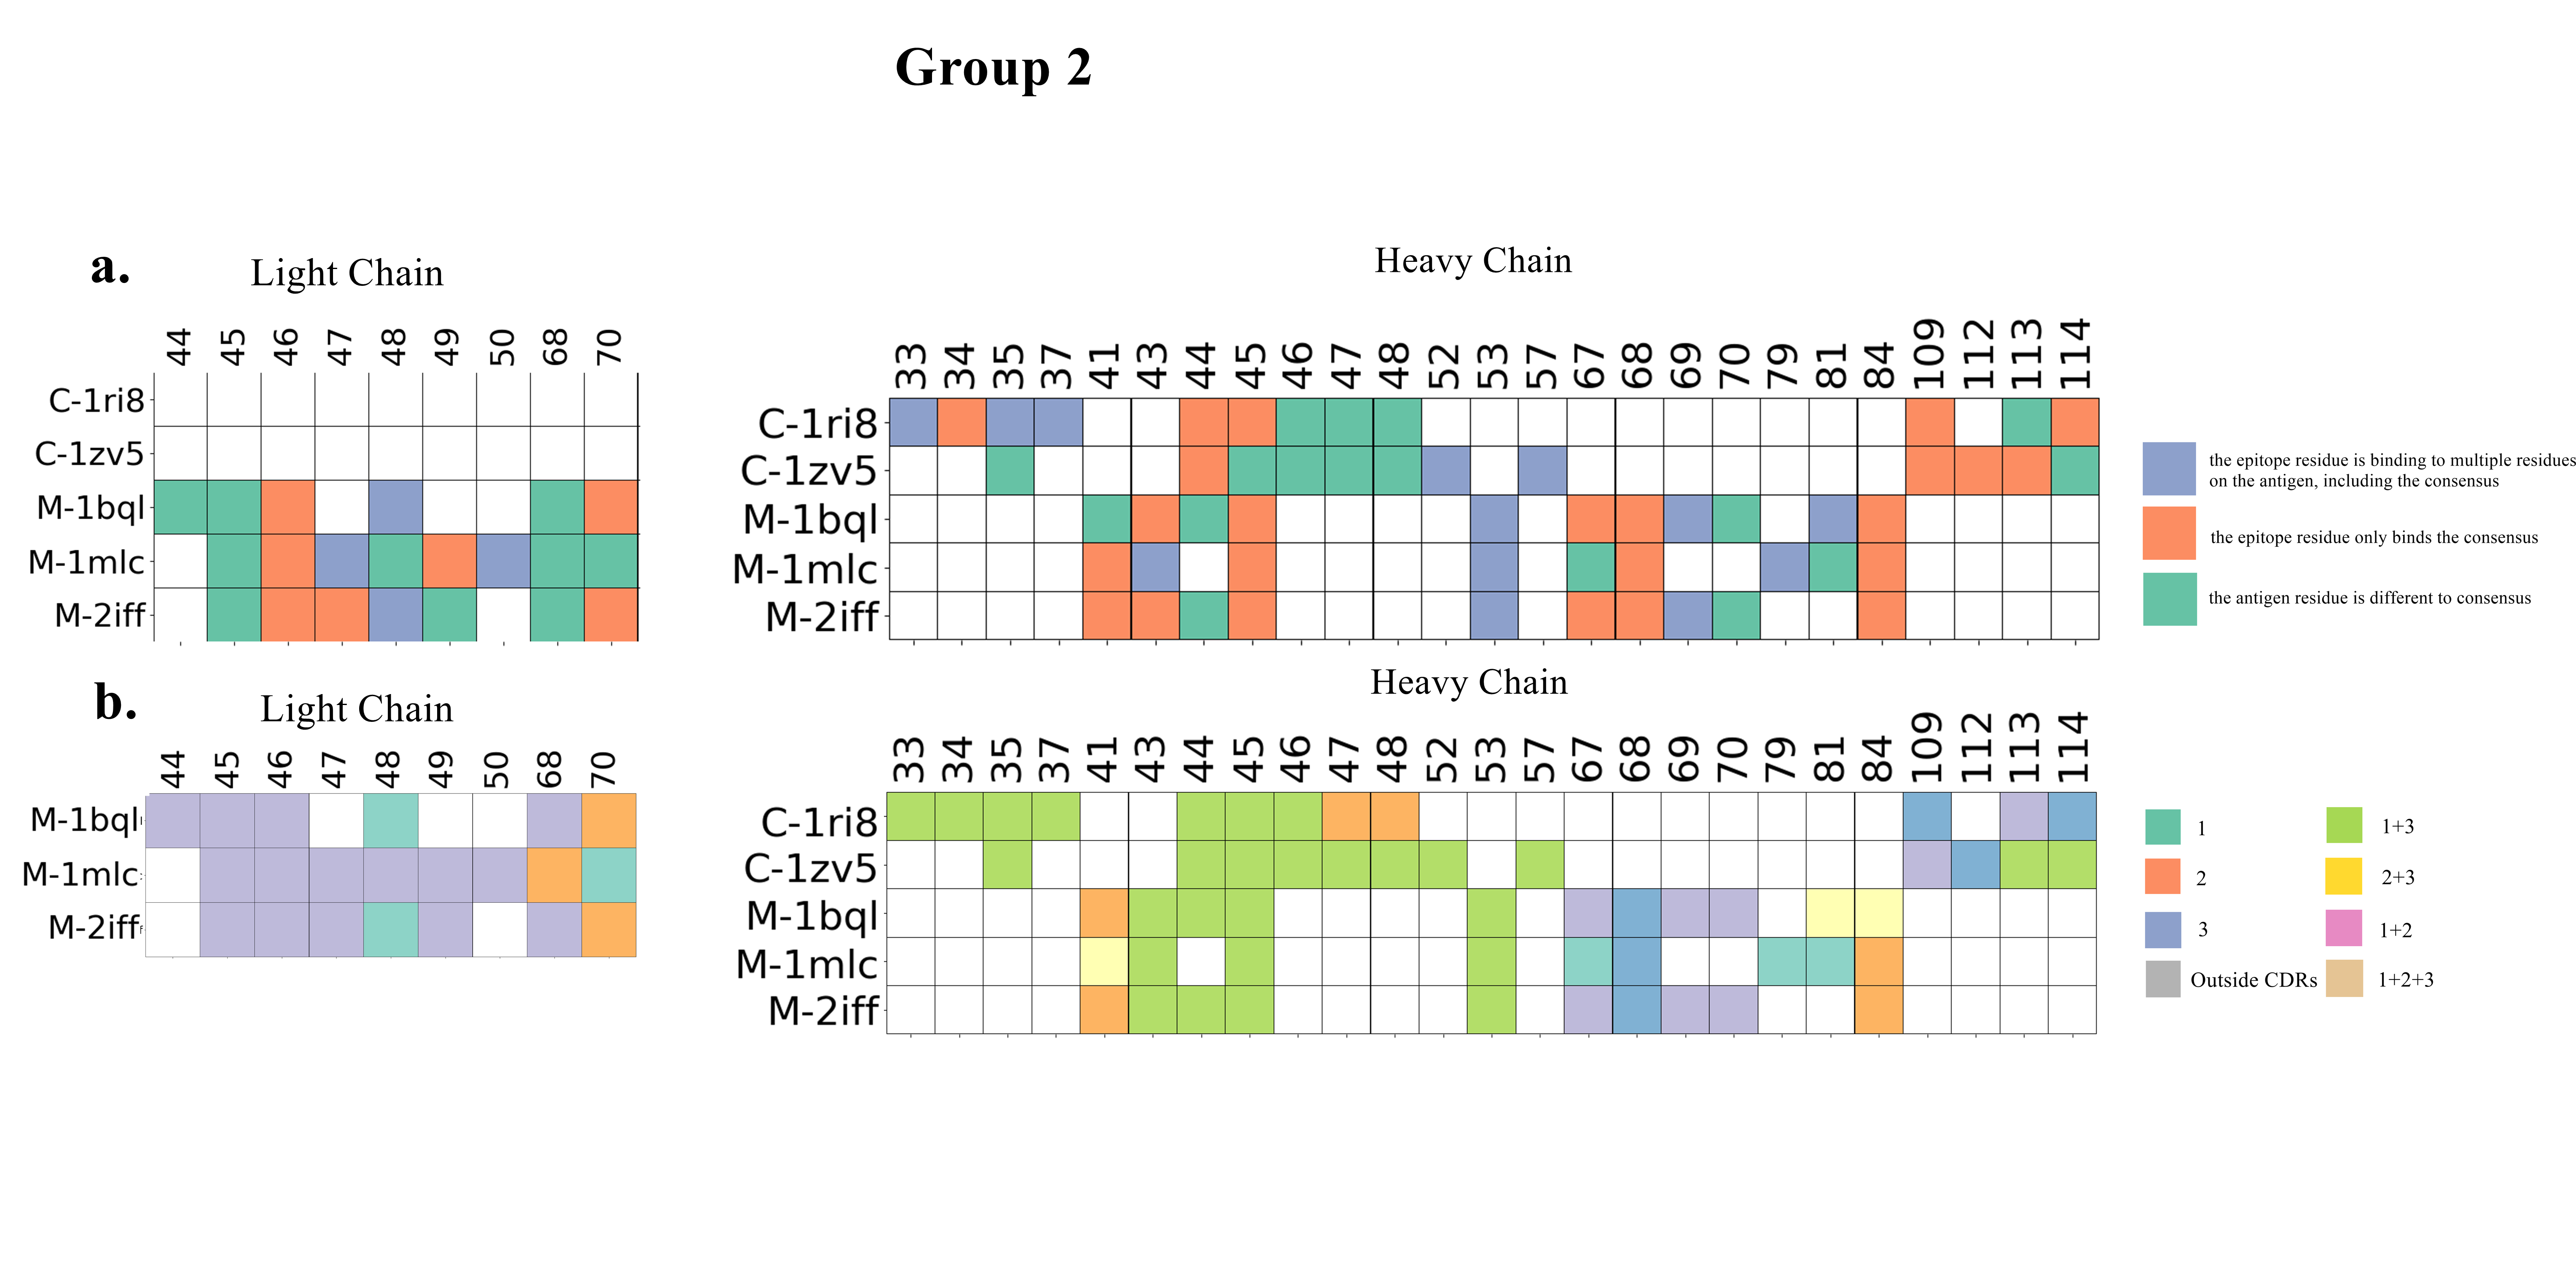
\includegraphics[width=0.99\linewidth]{plots_new_gr/g2_CDR_light_vs_heavy_101}
	\caption{}
	\label{fig:g2cdrlightvsheavy101}
\end{figure}
\begin{figure}[h]
	\centering
	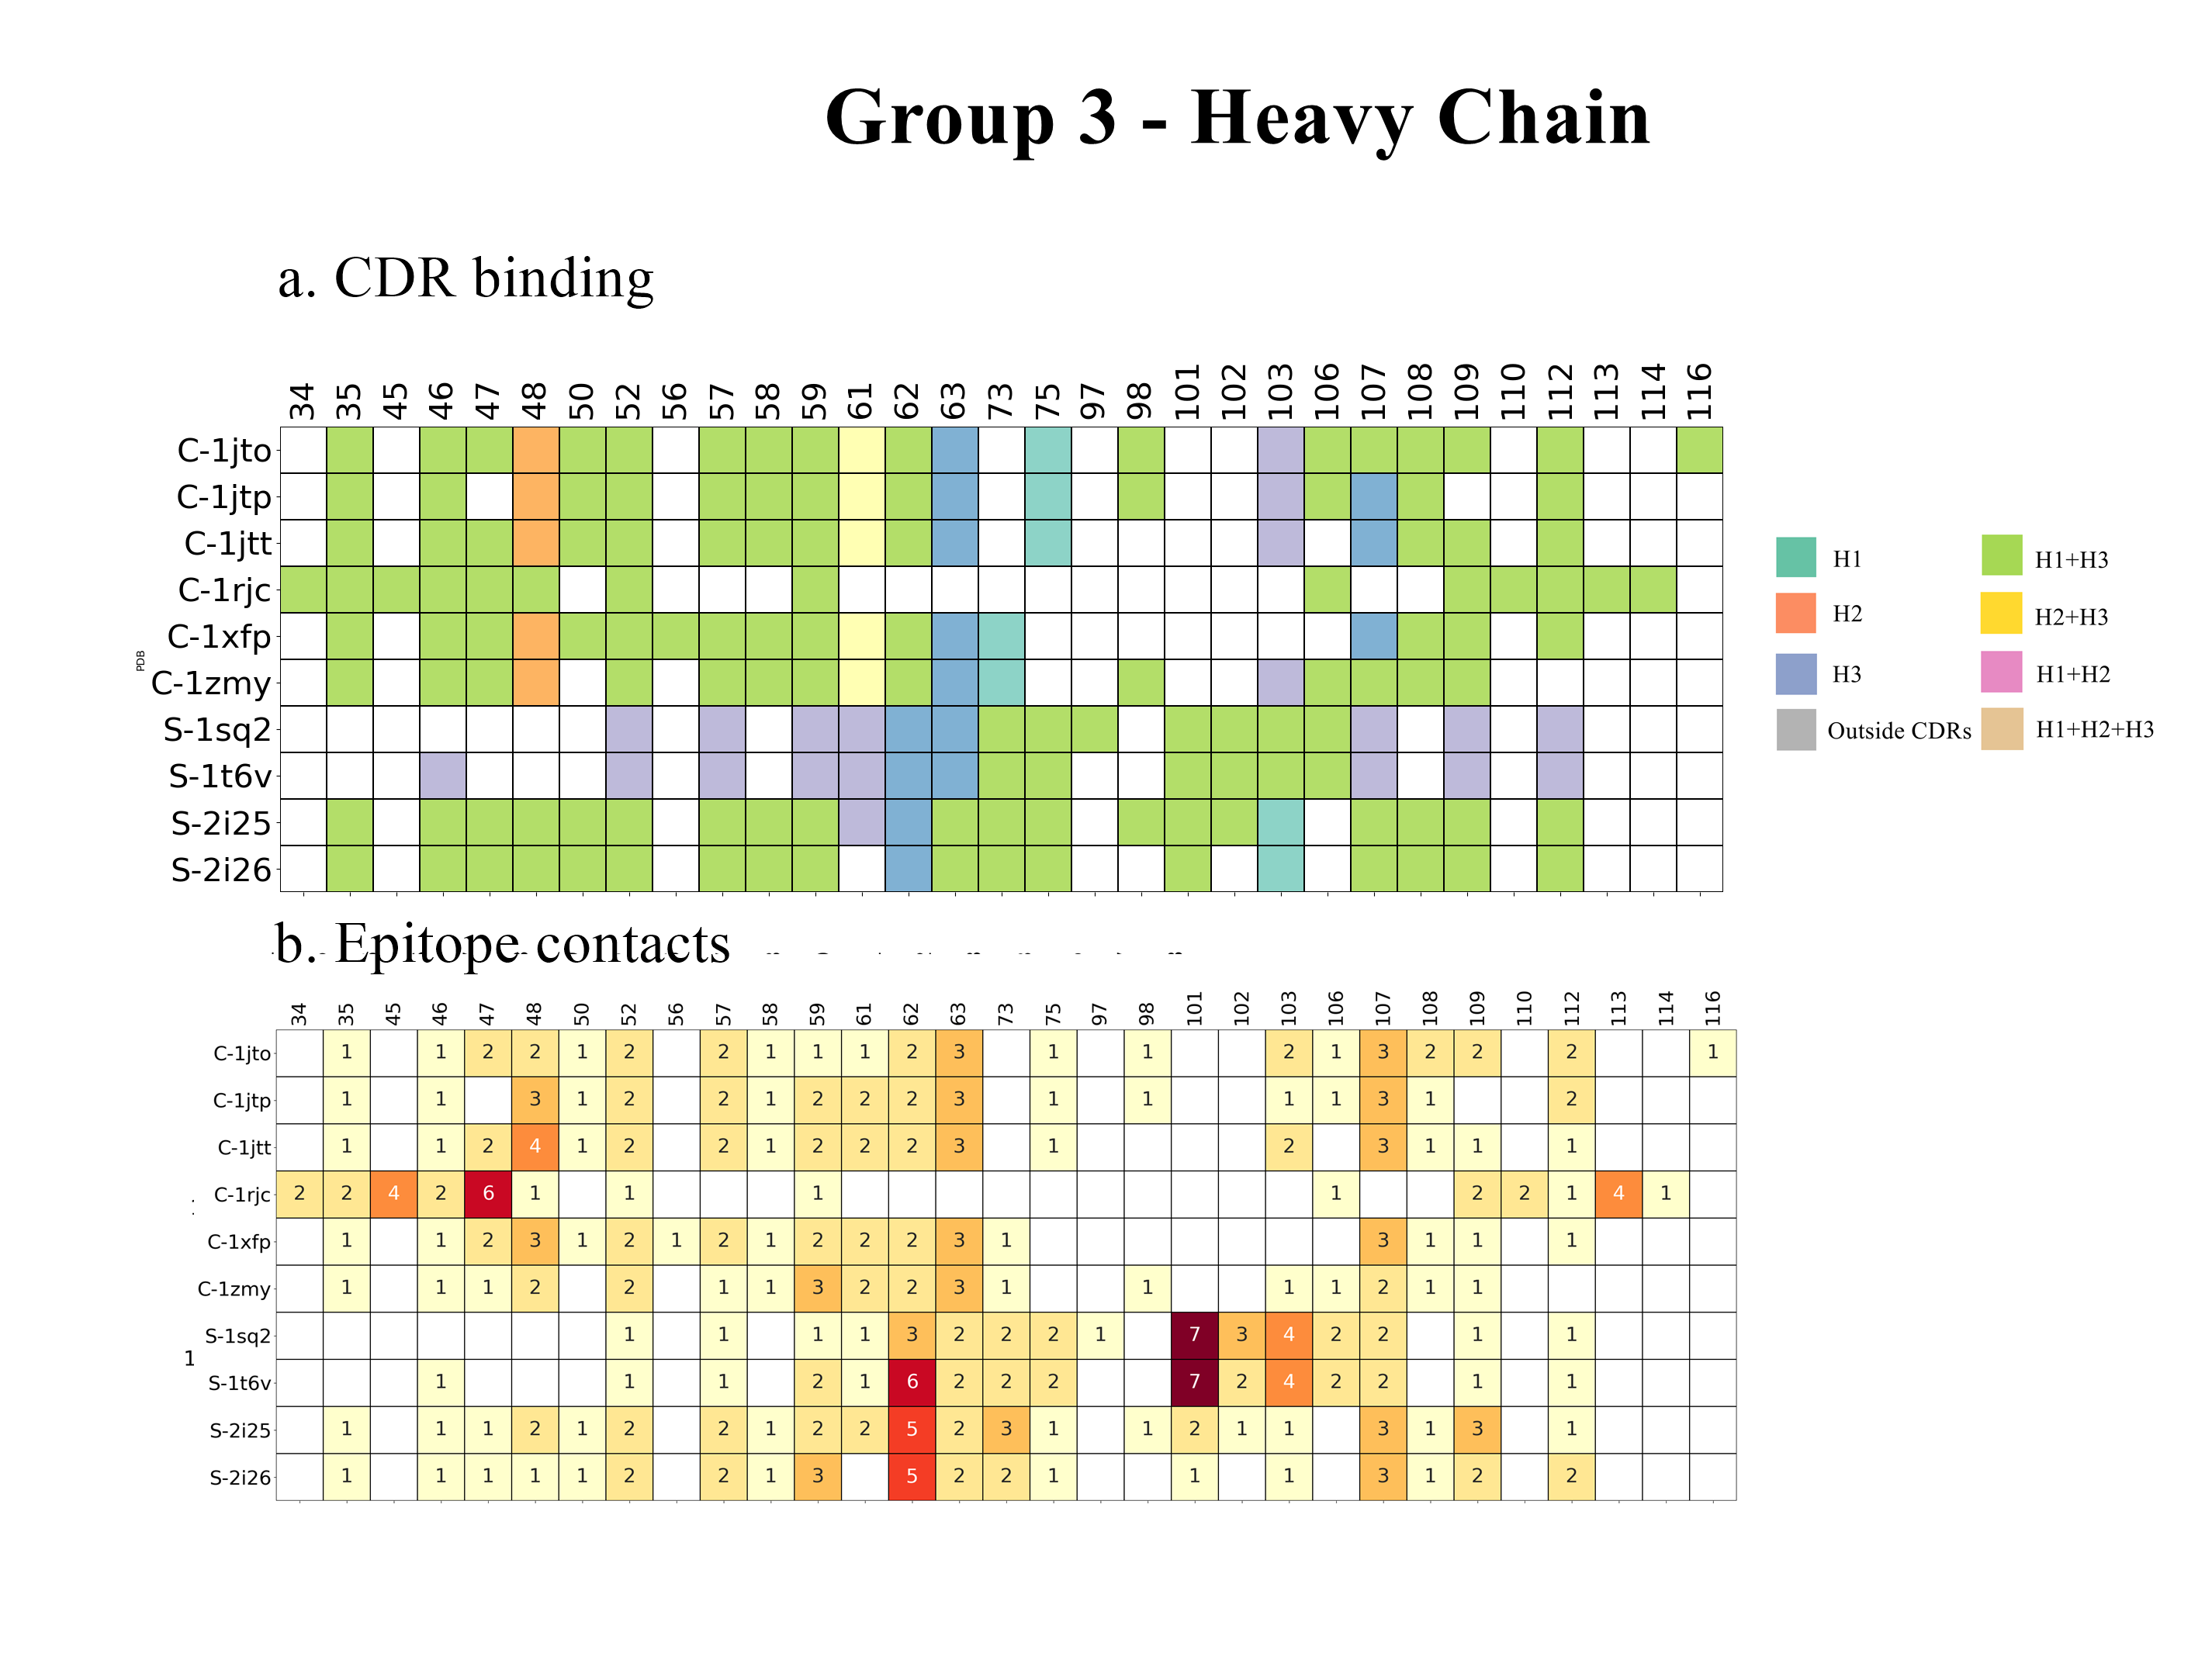
\includegraphics[width=0.7\linewidth]{plots_new_gr/gr3_cdr_vs_epitope}
	\caption{}
	\label{fig:gr3cdrvsepitope}
\end{figure}





\newpage

CDRS

the Heavy chains are more variable than the light chains(42 unique vs 25 unique)
\end{document}
